%! TEX root = 'main.tex'
\section{Case Study}
\label{sec:casestudy}
In this section, we use an example to show how our CPU executes an instruction.
We designed a load instruction
\begin{lstlisting}
LDA mem4
\end{lstlisting}
This instruction indicates that the 4-bit operand is used as the memory address to read 1 byte of data into register A. For example, we want to load data from memory address 0xE, then the instruction is "LDA 0xE". Because the opcode of the LDA instruction is defined as 0x1, the binary form of this instruction is 0001 1110 (0x1E).

LDA instruction takes 4 clock cycle to finish.

\begin{enumerate}
	\item CO MI
	\item RO II CE
	\item IO MI
	\item RO AI
\end{enumerate}

In these four clock cycles, the first two can be regarded as the instruction fetch phase. These two cycles are the same in almost all the instructions we implemented.

Suppose the initial state of the CPU is as follows.

\begin{itemize}
	\item PC = 0x0
	\item Memory is initialized as in~\autoref{tab:memory}
\end{itemize}

\begin{table}[th]
	\begin{tabular}{|c|c|c|c|c|c|c|c|c|c|c|c|c|c|c|c|} 
		\hline
		0x0 & 0x1 & 0x2 & 0x3 & ...  & 0xB & 0xC & 0xD & 0xE & 0xF \\ 
		\hline
		0x1E & 0 & 0 & 0 & ... & 0 & 0 & 0 & 0xA & 0 \\
		\hline
	\end{tabular}
	\caption{Memory}
	\label{tab:memory}
\end{table}

The program counter points to the beginning of the memory, which stores the instruction binary 0x1E. At memory 0xE, which is the position to be read by this instruction, there is data 0xA.

\subsection{Clock Cycle 1}

We issue two control signals.

\begin{itemize}
	\item CO (COUNTER OUT)
	\item MI (MAR IN)
\end{itemize}


By issuing these two control signals, the PC sends its 4-bit value to the bus, and the MAR get the 4-bit value from the bus, as shown in~\autoref{fig:cc1}.

\begin{figure}[th]
	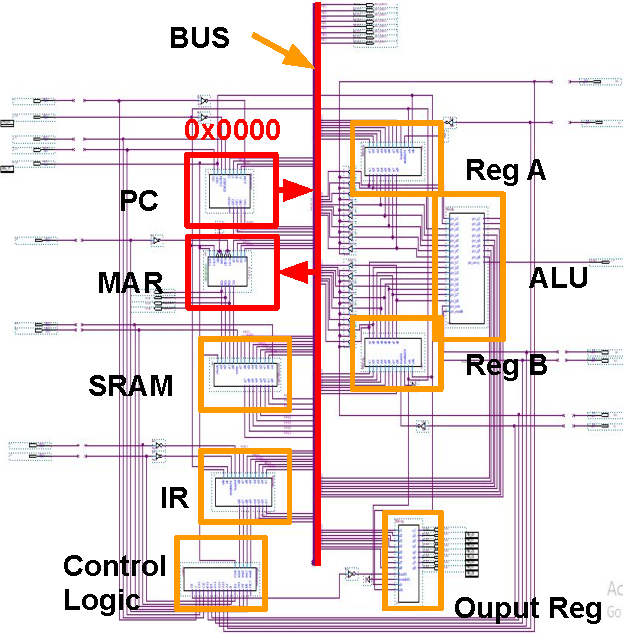
\includegraphics[width=0.47\textwidth]{figures/cc1}
	\centering
	\caption{Clock Cycle 1}
	\label{fig:cc1}
\end{figure}

As a result, the value in the PC is sent to the MAR and now MAR is 0x0.


\subsection{Clock Cycle 2}

We issue three control signals.

\begin{itemize}
	\item RO (RAM OUT)
	\item II (IR IN)
	\item CE (COUNTER ENALBE)
\end{itemize}

By issuing RO and II, the RAM sends the byte to the bus and the IR gets it, as shown in~\autoref{fig:cc2}. CE is also issued at this clock cycle, so the PC will increase one.

\begin{figure}[th]
	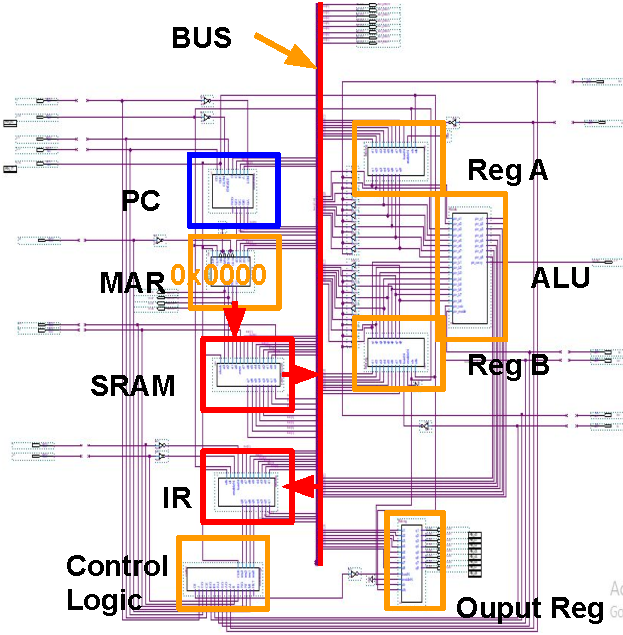
\includegraphics[width=0.47\textwidth]{figures/cc2}
	\centering
	\caption{Clock Cycle 2}
	\label{fig:cc2}
\end{figure}

As a result, the instruction is successfully loaded into the IR. Now IR contains value 0x1E.


\subsection{Clock Cycle 3}

We issue two control signals.

\begin{itemize}
	\item IO (IR OUT)
	\item MI (MAR IN)
\end{itemize}

This clock cycle can be viewed as the decoding phase. When IO is signaled, as mentioned earilier, the data in the IR is divided into two parts, the lower 4 bits are sent to the bus, and the upper 4 bits are send to the control logic, as shown in~\autoref{fig:cc3}.


\begin{figure}[th]
	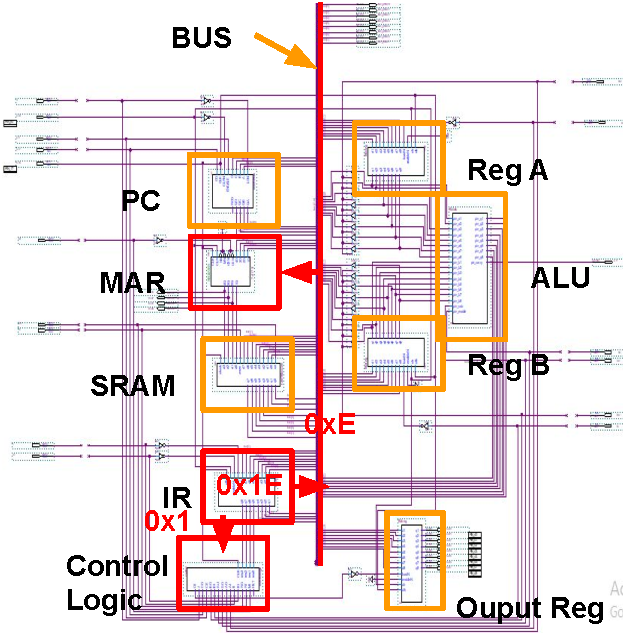
\includegraphics[width=0.47\textwidth]{figures/cc3}
	\centering
	\caption{Clock Cycle 3}
	\label{fig:cc3}
\end{figure}

As a result, the operand which is a memory address, now is loaded into MAR. MAR has 0xE and the control logic also gets the opcode.


\subsection{Clock Cycle 4}

We issue two control signals.

\begin{itemize}
	\item RO (RAM OUT)
	\item AI (A IN)
\end{itemize}

Because in the last clock cycle, the MAR already loaded with the memory address 0xE. In this clock cycle, the RO causes the memory to send the corresponding data to the bus. Meanwhile, register A gets data from the bus, as shown in~\autoref{fig:cc4}.

\begin{figure}[th]
	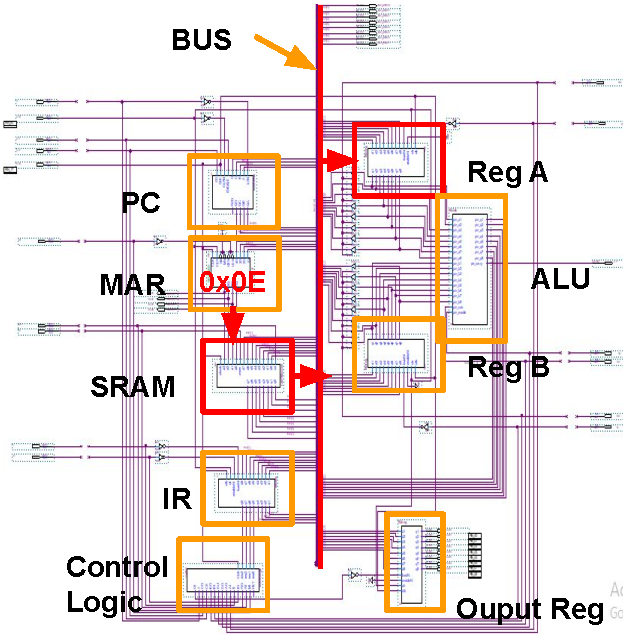
\includegraphics[width=0.47\textwidth]{figures/cc4}
	\centering
	\caption{Clock Cycle 4}
	\label{fig:cc4}
\end{figure}

So we see that when this clock cycle ends, the value in memory 0xE has been successfully loaded into register A. Now register A has the value 0xA.
